\documentclass[12pt,aspectratio=169]{beamer}
\usepackage{fancyvrb}
\RecustomVerbatimCommand{\VerbatimInput}{VerbatimInput}{frame=single,
numbersep=1mm, numbers=left, formatcom=\color{orange}}
%\usepackage{kpfonts}
%\usepackage[bitstream-charter]{mathdesign}
\usepackage[utf8]{inputenc}
\usepackage{pgf}
\usepackage{verbatim}
%\usepackage{fontspec}
\usepackage[ruled,vlined,linesnumbered]{algorithm2e}
\IncMargin{1em}
\usetheme{Madrid}
\setbeamerfont{frametitle}{series=\bfseries}
\usecolortheme[dark]{solarized}
\setbeamertemplate{blocks}[rounded][shadow=false]
\setbeamertemplate{navigation symbols}{}

\author{Gianluca Della Vedova}
\title[Advanced Algorithms]{Advanced Techniques for Combinatorial Algorithms:
Data Streams and Map-Reduce}
\institute[]{Univ. Milano--Bicocca\\
  \texttt{https://gianluca.dellavedova.org}}
\date[]{{\tiny \today\hspace{1em}}}

\DeclareMathOperator{\poly}{\text{poly}}
\DeclareMathOperator{\polylog}{\text{polylog}}


% If you wish to uncover everything in a step-wise fashion, uncomment
% the following command:
% \beamerdefaultoverlayspecification{<+->}

\begin{document}

\begin{frame}
  \titlepage
\end{frame}


\begin{frame}\frametitle{Gianluca Della Vedova}
  \begin{itemize}
  \item
                Advanced Techniques for Combinatorial Algorithms
\item
{\small\url{https://gitlab.com/dellavg/advanced-algorithms}}
  \item
{\small\url{https://gianluca.dellavedova.org}}
  \item
{\small\url{gianluca.dellavedova@unimib.it}}
  \end{itemize}
\end{frame}

\begin{frame}\frametitle{Fact 1}
  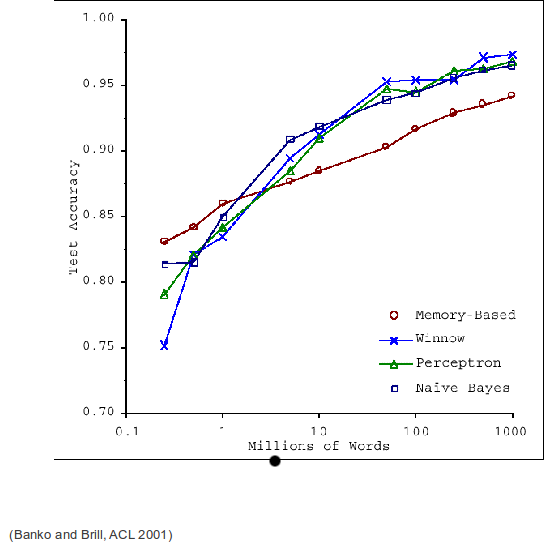
\includegraphics[width=5cm]{img/growing-data-1}
  \begin{itemize}
  \item
    Huge data are among us
  \end{itemize}
\end{frame}


\begin{frame}\frametitle{And more are coming}
  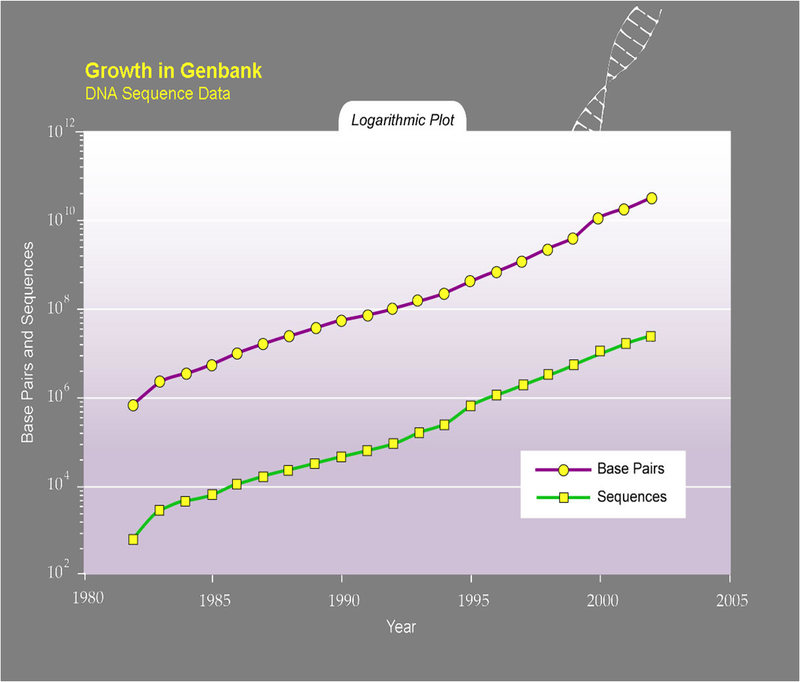
\includegraphics[width=6cm]{img/Kurzweil_DNA_Sequence_data_growth,_base_pairs_and_sequences_per_year}

  \small
  From 1982 to the present, the number of bases in GenBank has doubled
approximately every 18 months (\url{ftp://ftp.ncbi.nih.gov/genbank/gbrel.txt}).
\end{frame}



\begin{frame}\frametitle{Moore's Law}
  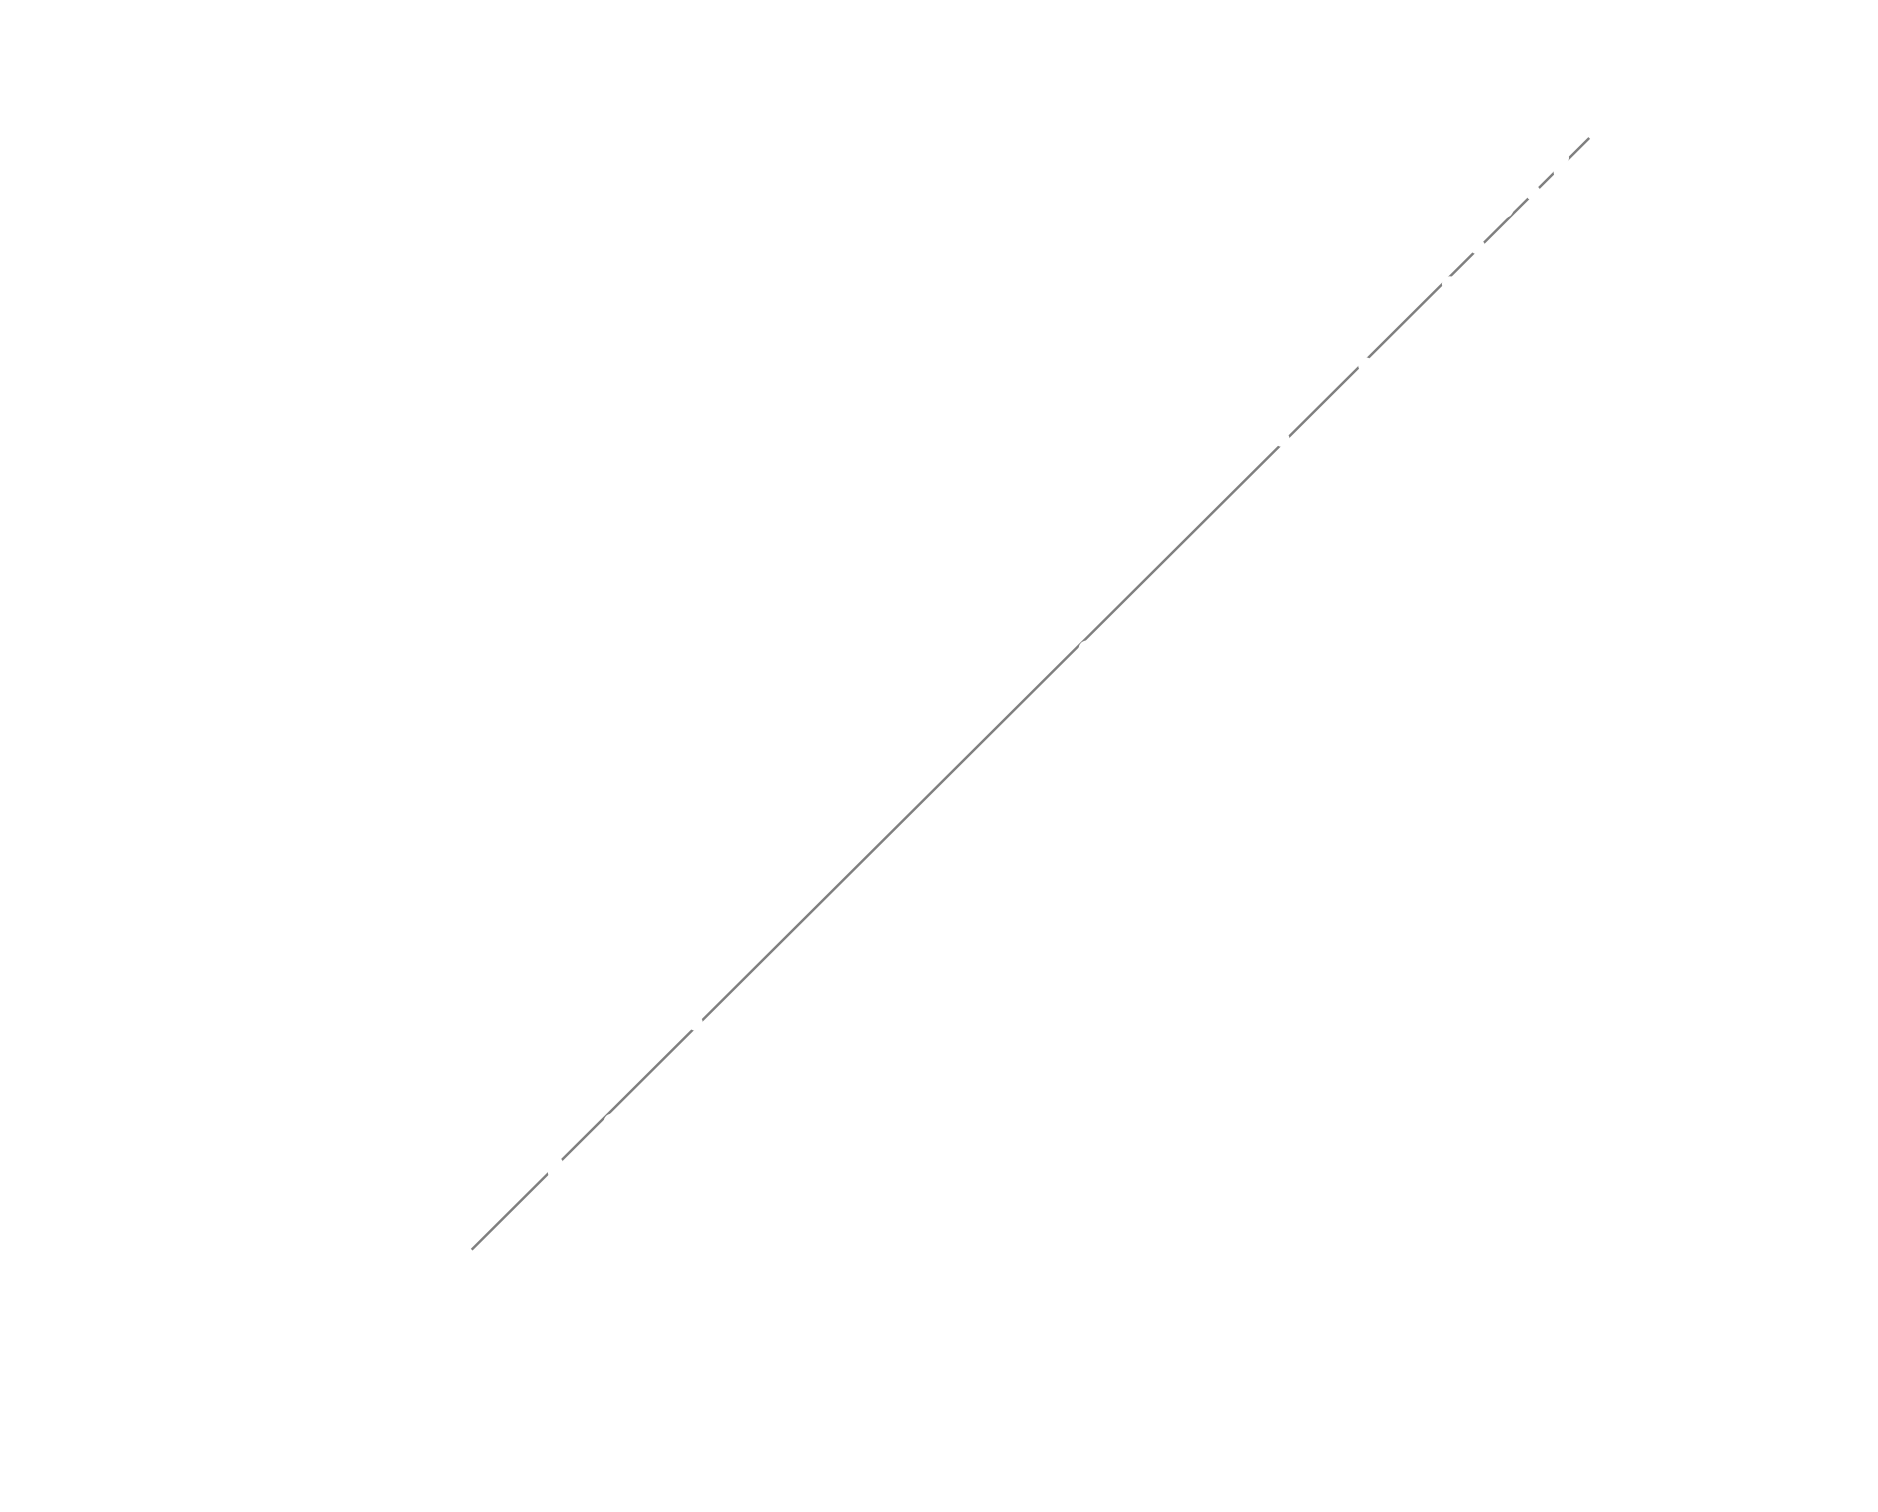
\includegraphics[width=8cm]{img/Moore_Law2}

  \tiny\url{https://en.wikipedia.org/wiki/File:Transistor_Count_and_Moore\%27s_Law_-_2011.svg}
\end{frame}





\begin{frame}\frametitle{Fact 2}
  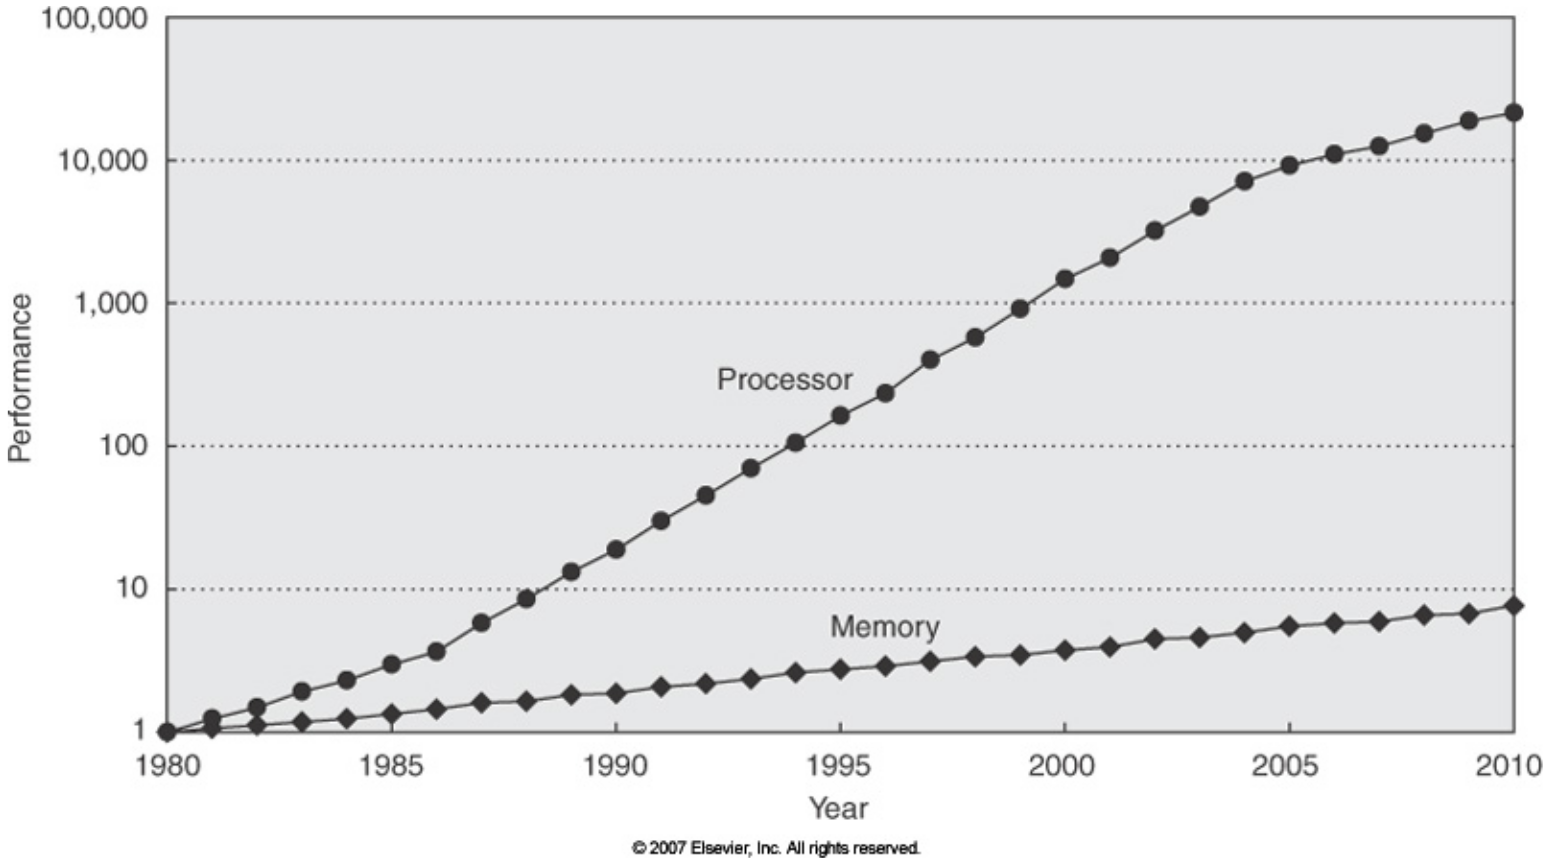
\includegraphics[width=10cm]{img/memory-cpu-gap}
  \begin{itemize}
  \item
    Moore's Law is unfair.
  \end{itemize}
\end{frame}


\begin{frame}\frametitle{Problem}
  \begin{itemize}
  \item
    Input data too large for a single computer
  \item
    Don't fit into memory
  \end{itemize}
\end{frame}

\begin{frame}\frametitle{Solution}
  \begin{itemize}
  \item
    Split data into parts
  \item
    If only it were so easy
  \item
    Embarassingly parallel problems
  \end{itemize}
\end{frame}

\begin{frame}\frametitle{Solutions}
  \begin{itemize}
  \item
    parallel algorithms
  \item
    map reduce
  \item
    data streaming
  \item
    External-memory algorithms
  \item
    Are all related
  \end{itemize}
\end{frame}


\section{Models}

\begin{frame}\frametitle{Map Reduce model}
  \begin{itemize}
  \item
    \alert{Input}: hash = $<$key $\mapsto$ value$>$ pairs
  \item
    Map
  \item
    Shuffle
  \item
    Reduce
  \item
    \alert{Output}: hash
  \end{itemize}
\end{frame}

\begin{frame}\frametitle{Map Reduce model}
  \begin{itemize}
  \item
    Mapper: receives
    \alert{a} $<$key $\mapsto$ value$>$ \alert{pair}, computes a hash\uncover<4-6>{ \textbf{in parallel}}
  \item
    Shuffle: \alert{all} values with \alert{same key} $k$ are assigned to a
    unique processor \uncover<5-6>{ \textbf{automatic}}
  \item
    Reducer: receives \alert{all} values with \alert{same value} $k$, computes
      a \alert{multiset} of     $<k,\text{value}>$ pairs \uncover<6>{
        \textbf{sequential algorithm on the values}}
  \end{itemize}
\end{frame}

\begin{frame}\frametitle{$k$-th Frequency Moment }
\begin{columns} 
  \begin{column}{0.48\textwidth}
  \begin{block}{Instance}
    $k$, a list $L=\langle x_{1}, \ldots, x_{n} \rangle$ of elements over alphabet $\Sigma$
  \end{block}
  \begin{block}{Output}
    $\sum_{\sigma\in\Sigma} f^{k}(\sigma)$, where $f(\sigma)$ is the number of occurrences
    of $sigma$ in $L$
  \end{block}
\end{column}
    
\begin{column}{0.48\textwidth}
      \begin{block}{Example}
        $L=\langle 0,1,1,1,2,0,1,2,0,1,1,2\rangle$
      \end{block}
      \begin{block}{Output, $k=2$}
        $3^{2}+6^{2}+ 3^{2} =54$
      \end{block}
    \end{column}
\end{columns}
\end{frame}




\begin{frame}\frametitle{Example: $k$-th frequency moment}
\begin{algorithm}[H]
\KwData{$k$, a list  $=L\left\langle x_{1}, \ldots , x_{n} \right\rangle $}

$\mu_{1}(\langle i; x_{i} \rangle) = \langle x_{i}; i \rangle$\tcc{$i$ is the index}

$\rho_{1}  (\langle x_{i} ; {v_{1} , \ldots , v_{m}} \rangle) = \langle x_{i} ;
m^{k}\rangle$\tcc*{All occurrences of a symbol are grouped together}

$\mu_{2}(\langle x_{i} ; v \rangle) = \langle \$ ; v \rangle$ \tcc*{Time to sum}

$\rho_{1}  (\langle \$ ; {v_{i} , \ldots , v_{l}} \rangle) = \left\langle \$
; \sum v_{i} \right\rangle $\;
\caption{$k$-FrequencyMoment}
\end{algorithm}
\end{frame}

\begin{frame}\frametitle{Rationale}
\begin{itemize}
\item
  No machine can store whole input
\item
  Too many machines = \alert{bad}
\item
  Shuffling is expensive
\item
  No shared memory
\item
  Loose synchronization
\end{itemize}
\end{frame}

\begin{frame}\frametitle{Efficient Algorithm}
\begin{itemize}
\item
  at most  $O(n^{1-\epsilon})$ machines
\item
  each mapper is a RAM with $O(n^{1-\epsilon})$ space, $\poly(n)$ time
\item
  each reducer is a RAM with $O(n^{1-\epsilon})$ space, $\poly(n)$ time
\item
  polylogarithmic mapreduce rounds
\item
  reducers have $O(n^{2-2\epsilon})$ overall space
\item
  each key has $O(n^{1-\epsilon})$ values
\end{itemize}
\end{frame}

\begin{frame}\frametitle{Classes}
\begin{itemize}
\item
$\mathcal{MRC}^{i}$ if $O(\log^{i}n)$ rounds
\item
$\mathcal{MRC} = \bigcup_{i=0}^{\infty}\mathcal{MRC}^{i}$
\item
$\mathcal{MRC}^{0}$, $\mathcal{MRC}^{1}$
\end{itemize}
\end{frame}

\begin{frame}\frametitle{Map Reduce model}
Howard J. Karloff, Siddharth Suri, Sergei Vassilvitskii: A Model of Computation for MapReduce. SODA 2010: 938-948
\end{frame}


% \begin{frame}\frametitle{Massively Unordered Distributed (MUD)}
%   \begin{itemize}
%   \item
%     Reducer receives a \alert{stream} of values
%   \item
%     Reducer has $\polylog(n)$ space
%   \item
%     Feldman, Muthukrishnan, Sidiropoulos, Stein, Svitkina.
%  On Distributing Symmetric Streaming Computations.
% ACM Transactions on Algorithms~6(4):art.~66, 2010.
%   \end{itemize}
% \end{frame}


% \begin{frame}\frametitle{Memory Hierarchy}
%   \begin{itemize}
%   \item
%     CPU Registers
%   \item
%     L1 Cache: $32-256$ KBytes, latency $< 10^{-9}$ secs
%   \item
%     L2 Cache: $1-16$ MBytes, block transfer size $B=32$ Bytes
%   \item
%     RAM: $1-32$ GBytes,  $B=64$ Bytes
%   \item
%     Disk: $100$ GBytes - $1$ PBytes,  $B=8$ KBytes, latency $> 10^{-3}$ secs
%   \end{itemize}
% \end{frame}



  \section{Relations between models}
\begin{frame}\frametitle{}
  \begin{center}
    \Huge
    Relations between models
  \end{center}
\end{frame}

\begin{frame}\frametitle{Map Reduce and PRAM}

\begin{block}{Reconcile inputs}
  $x_{1}, \ldots , x_{n} \mapsto \left\langle 1, x_{1} \right\rangle, \ldots ,
\left\langle n,x_{n} \right\rangle $
\end{block}

\begin{block}{Theorem 4.1, Karloff et al, SODA 2010}
  If $\mathcal{P} \neq \mathcal{NC}$ then $\mathcal{MRC} \not\subseteq
  \mathcal{NC}$.
\end{block}

\begin{block}{Proof}
  \begin{itemize}
  \item
    Pick a $\mathcal{P}$-complete problem, and pad its input
  \item
    Use a single reducer to solve it
  \end{itemize}
\end{block}
\end{frame}


\begin{frame}\frametitle{Map Reduce and PRAM}
\begin{block}{Theorem 7.1, Karloff et al, SODA 2010}
Any CREW PRAM algorithm using
$O(n^{2-2\epsilon})$ total memory, $O(n^{2-2\epsilon})$ processors and $t(n)$
time can be run in $O(t(n))$ rounds in $\mathcal{MRC}$.
\end{block}

\begin{block}{Proof}
  \begin{itemize}
  \item
    processor $\to$ reducer
  \item
    memory location $\to$ reducer
  \item
    shuffle to coordinate read requests
  \end{itemize}
\end{block}
\end{frame}


% \begin{frame}\frametitle{MUD and PRAM}
% \begin{block}{Theorem 4.1, Feldman et al, ACM Trans.
%  Alg. 2010}
% Any $N$-processors, $M$-memory, $T$-time EREW PRAM algorithm can be simulated
% by a $O(T)$-round $(N+M)$-key MUD algorithm.
% \end{block}

% \begin{block}{Corollary}
%   Any problem in $\mathcal{NC}$ has a $\polylog(n)$-round, $\poly(n)$-key MUD
%   algorithm with communication complexity $O(\log(n))$ bits per key.
% \end{block}
% \end{frame}


\begin{frame}\frametitle{Map Reduce and PDM}
  \begin{block}{Shuffle step}
  \begin{itemize}
  \item
    Matrix: $R$=rows=reduce steps, $M$=columns=keys
  \item
    sparse matrix
  \item
    Layout depending on maps
  \item
    Rearrange into a column-wise ordering
  \end{itemize}
\end{block}
\end{frame}



\section{Algorithms}



\begin{frame}\frametitle{Graph Algorithms}
  \begin{itemize}
  \item
    For each edge $e$, store its successor $s(e)$
  \item
    Euler tour of $G$ = edge-disjoint cycles
  \item
    merge any two cycles with a common vertex $u$
  \end{itemize}
\end{frame}

\begin{frame}\frametitle{Minimum Spanning Tree (MRC)}
  \begin{algorithm}[H]
    \KwData{Array}{dense graph $G=\left\langle V,E \right\rangle $}

    \tcc{$|V|=n$, $|E|\ge n^{1+c}$}
    $V_{1}, \ldots, V_{k} \gets $ random balanced partition of $V$\;
    $E_{i,j} \gets \{(u, v) \in E | u, v \in V_{i} \cup V_{j} \}$\;
    $G_{i,j} \gets $ subgraph of $G$ induced by $E_{i,j}$\;
    \ForEach{$G_{i,j}$}{
      $M_{i,j}\gets $ minimum spanning forest of $G_{i,j}$
    }
    $H \gets \left\langle V, \bigcup_{i,j} M_{i,j}\right\rangle $\;
    $M \gets$ minimum spanning tree of $H$\;
    \label{alg:MRC-MST}
    \caption{MST}
  \end{algorithm}
\end{frame}

\begin{frame}\frametitle{Minimum Spanning Tree (MRC)}
  \begin{block}{MST Algorithm is correct}
    \begin{enumerate}
      \item
    Let $e\in E\setminus E(H)$.
      \item
    Then $e$ is a heaviest edge in some cycles of $G_{i,j}$.
      \item
    The same cycle is also in $G$.
  \end{enumerate}
\end{block}
\end{frame}



\begin{frame}\frametitle{Minimum Spanning Tree (MRC)}
  \begin{block}{$k = n^{c/2}$.    Then $|E_{i,j}|$ is $\tilde{O}(n^{1+c/2})$}
    \begin{enumerate}
      \item
        $W_{i} = \{v \in V : 2^{i-1} < deg(v) \le 2^{i} \}$
      \item
        If $|W_{i} | < 2n^{c/2}\log n $ then $\sum_{v\in W_{i}}\text{deg}(v) =
        \tilde{O}(n^{1+c/2})$
      \item
        Else $|W_{i} \cap V_{j}| = O(\log n)$ via Chernoff bound.
        Proof completed via union bound
      \end{enumerate}
    \end{block}

    \begin{block}{Chernoff bound}
    \begin{enumerate}
      \item
      $X=\sum_{i}^{q}X_{i}$, $X_{i}$ ind. random variables, $Pr[X_{i}=1]=Pr[X_{i}=-1]=1/2$
    \item
      $Pr[X\ge a] \le e^{\frac{-a^{2}}{2q}}$
    \end{enumerate}
  \end{block}
\end{frame}


\begin{frame}\frametitle{MRC General Technique}
  \begin{block}{Def. $f$ parallelizable function}
    \begin{enumerate}
    \item
      If there exists functions $g, h$ such that:
    \item
      For any partition $T_{i}, \ldots , T_{k}$ of the universe set $S$, $f(S)
      = h(g(T_{1}), \ldots , g(T_{k}))$
    \item
      $g, h$ are polynomial time computable
    \item
      Output of $g$ has $O(\log n)$ bits.
    \end{enumerate}
  \end{block}

  \begin{block}{$\mathcal{MRC}$ algorithm for $f_{1}, \ldots, f_{k}$}
    \begin{enumerate}
    \item
      $S_{1}, \ldots , S_{k}$ subsets of $S$, $k\le n^{2-3\epsilon}$, $\sum
      |S_{i}|\le n^{2-2\epsilon}$
    \item
      $f_{1}(S_{1}), \ldots , f_{k}(S_{k})$ with $O(n^{1-\epsilon})$ reducers,
      $O(n^{1-\epsilon})$ space each.
    \end{enumerate}
  \end{block}
\end{frame}

\begin{frame}\frametitle{$k$-th frequency moment}
\begin{algorithm}[H]
\KwData{$k$, a sequence $\left\langle x_{1}, \ldots , x_{n} \right\rangle $}

$\mu_{1}(\langle i; x_{i} \rangle) = \langle x_{i}; i \rangle$\;

$\rho_{1}  (\langle x_{i} ; {v_{i} , \ldots , v_{m}} \rangle) = \langle x_{i} ;
m^{k}\rangle$\;

$\mu_{2}(\langle x_{i} ; v \rangle) = \langle \$ ; v \rangle$\;

$\rho_{1}  (\langle \$ ; {v_{i} , \ldots , v_{l}} \rangle) = \left\langle \$
; \sum v_{i} \right\rangle $\;
\caption{$k$-FrequencyMoment}
\end{algorithm}
\end{frame}


\begin{frame}\frametitle{$k$-th frequency moment}
  \begin{block}{Problem: all elements can be the same}
      $O(n)$ space, instead of $O(n^{1-\epsilon})$
    \end{block}

  \begin{block}{Solution}
    \begin{itemize}
    \item
      $g(\{t_{1}, \ldots , t_{k} \}) = k$
    \item
      $h(\{i_{1}, \ldots , i_{m} \}) = (i_{1} + \cdots + i_{m} )^{k}$
    \end{itemize}
  \end{block}

  \begin{block}{Proof}
    \begin{itemize}
    \item
      $h(g(T_{1}), \ldots , g(T_{m})) = |S|^{k}$
    \item
      $S$ set of pairs with same value
    \end{itemize}
  \end{block}
\end{frame}


% \begin{frame}\frametitle{Minimum Spanning Tree 2 (MRC)}
%   \begin{algorithm}[H]
%     \KwData{Array}{dense graph $G=\left\langle V,E \right\rangle $}

%     $\beta\gets O(|E|)/\eta$\; \tcc{$\eta$: memory size}
%     $E_{1}, \ldots, E_{\beta} \gets $ random partition of $E$ into $\beta$ sets\;
%     \ForEach{$G_{i,j}$ in parallel}{
%       $T_{i}\gets $ Min spanning forest on $E_{i}$
%     }
%     Return($\left\langle V, \bigcup T_{i} \right\rangle$ )
%     \label{alg:MRC-MST2}
%     \caption{MST2}
%   \end{algorithm}
% \end{frame}


\begin{frame}\frametitle{Maximal Matching (MRC)}
  \begin{block}{Matching}
    \begin{itemize}
    \item
      Let $G=\left\langle V,E \right\rangle $ be a graph.
    \item
      Then $M\subseteq E$ is a matching if no two edges of $M$ shares a vertex
    \item
      $M$ is maximal if $\not\exists M_{1}\supseteq M$ s.t. $M_{1}$ is a matching
    \end{itemize}
  \end{block}
\end{frame}

\begin{frame}\frametitle{Maximal Matching (MRC)}
  \begin{algorithm}[H]
    \KwData{Array}{dense graph $G=\left\langle V,E \right\rangle $}

    $M\gets \emptyset$, $S=E$\;

    $E'\gets$ random sample of $S$\;
    \lIf{$|E'|>\eta$}{Fail}
    $M'\gets$ maximal matching on $E'$ \tcc{1 reducer}
    $M\gets M\cup M'$\;
    Remove all edges conflicting with $M$\;
    $S\gets $ remaining edges\;
    \lIf{$|I|>\eta$}{go to step 2}
    $M'\gets$ maximal matching on $M'$ \tcc{1 reducer}
    $M\gets M\cup M'$\;
    \label{alg:MRC-MC2}
    \caption{MaximalMatching}
  \end{algorithm}
\end{frame}

\begin{frame}\frametitle{Connected components}
  \begin{algorithm}[H]
    Label each vertex either \alert{up} or \alert{down}\;
    \ForEach{edge $(v,w)$}{
      Add the component of the down vertex to that of the up vertex\;
      \tcc{The root of the lower component is now a child of the root of the
        upper component}
    }
    \ForEach{vertex $v$}{
      parent[$v$] $\gets$ parent[parent[$v$]]
    }
    \caption{ConnectedComponents}
  \end{algorithm}
\end{frame}


\begin{frame}[fragile]\frametitle{Connected components}
  \begin{verbatim}
def map(u, v, p1, p2):
  if p1 == p2: #same component
    return []  #do nothing
  else:
    h1 = hash(p1, r)%2
    h2 = hash(p2, r)%2
    if h1 != h2:
      return [(p1,p2) if h1 else (p2,p1)]

def reduce(list):
  return list[0]
\end{verbatim}
\end{frame}


\begin{frame}\frametitle{Additional Bibliography on Map Reduce}
\small
On distributing symmetric streaming computations
\url{http://portal.acm.org/citation.cfm?doid=1824777.1824786}

Counting triangles and the curse of the last reducer
\url{http://portal.acm.org/citation.cfm?doid=1963405.1963491}

A Model of Computation for MapReduce \url{http://dl.acm.org/citation.cfm?id=1873677}
\end{frame}

\begin{frame}\frametitle{Data Streams}
  \begin{block}{Almost permutation}
    \begin{itemize}
    \item
      Input: a permutation $\pi$ of $\{1, \ldots , n\}$ with one element missing
    \item
      Find the missing element
    \item
      Streaming: read the input once
    \item
      $\lceil \log n \rceil$ bits of memory
    \end{itemize}
  \end{block}
\end{frame}  

\begin{frame}\frametitle{Almost permutation}
  \begin{block}{Algorithm}
    \begin{itemize}
    \item
      Keep the parity bits
    \item
      and add $\sum_{i=1}^{n} i$
    \end{itemize}
  \end{block}
\end{frame}

\begin{frame}\frametitle{Reservoir sampling}
  \begin{itemize}
  \item
    Take $k$ elements from a stream
  \item
    Add to $S$ the first $k$ elements
  \item
    The $i$-th elements is kept with probability $k/i$
  \item
    In case, remove a random element of $S$
  \end{itemize}
  \begin{block}{Uniform sampling}
    Time $t$, $i\le t$.
%
    Then $Pr[x_{i}\in S] = \frac{s}{t}$
  \end{block}
\end{frame}

\begin{frame}\frametitle{Count-Min sketch}
  \begin{itemize}
    \item
      Turnstile model
    \item
    Approximate counting: number of occurrences of a symbol
  \item
    $d\times w$ matrix  $count[]$
  \item
    $w=e/\epsilon$, $d=\log 1/\delta$.
We want additive error $\le\epsilon$ with probability $\ge 1-\delta$
  \item
    $d$ hash functions $h_{1}, \ldots h_{d}: \{1, \ldots, N\}\mapsto \{1, \ldots , w\}$
  \item
    update $(j, I_{i})$, then $count[k, h_{k}(j)] \gets count[k, h_{k}(j)] + I_{i}$,
    $\forall k$
  \item
    query $A[i]$, answer $\min_{j} count[j, h_{j}(i)]$
  \end{itemize}
\end{frame}

\begin{frame}\frametitle{HyperLogLog sketch}
\begin{itemize}
\item
    Estimate the cardinality of a set of integers
\item
    $p\gets$ Max number of leading zeroes
\item
    Estimate $2^{p}$
\item
    Go through hash function to manage arbitrary sets
\item
    Split into subsets to reduce variance
\end{itemize}
\end{frame}

\end{document}

%%% Local Variables:
%%% mode: latex
%%% TeX-PDF-mode: t
%%% buffer-file-coding-system: utf-8
%%% End:
